% THIS IS A LATEX TEMPLATE FILE FOR PAPERS INCLUDED IN THE
% *Anthology of Computers and the Humanities*. ADD THE OPTION
% 'final' WHEN CREATING THE FINAL VERSION OF THE PAPER. 
% DO NOT change the documentclass
\documentclass[final]{anthology-ch} % for the final version
%\documentclass{anthology-ch}         % for the submission

% LOAD LaTeX PACKAGES
\usepackage{booktabs}
\usepackage{graphicx}
\usepackage{hyperref}
\usepackage{minted}


% ADD your own packages using \usepackage{}

% TITLE OF THE SUBMISSION
% Change this to the name of your submission
\title{Historical data visual exploration meets static web technologies}

% AUTHOR AND AFFILIATION INFORMATION
% For each author, include a new call to the \author command, with
% the numbers in brackets indicating the associated affiliations 
% (next section) and ORCID-ID for each author.  
\author[1]{Paul Girard}[
  orcid=0000-0001-9332-3308
]
\affiliation{1}{OuestWare, Nantes, France}

% KEYWORDS
\keywords{Historical map, Vector map, Static web, Art History}

% METADATA FOR THE PUBLICATION
% This will be filled in when the document is published; the values can
% be kept as their defaults when the file is submitted
\pubyear{2025}
\pubvolume{2}
\pagestart{25}
\pageend{31}
\conferencename{Digital Humanities Tech Symposium 2025}
\conferenceeditors{Julia Damerow and Rebecca Sutton Koeser}
\doi{10.63744/K0GZLdLczoqm}

\addbibresource{bibliography.bib}

%%%%%%%%%%%%%%%%%%%%%%%%%%%%%%%%%%%%%%%%%%%%%%%%%%%%%%%%%%%%%%%%%%%%%%%%%%%
% HERE IS THE START OF THE TEXT

\begin{document}
\maketitle
\begin{abstract}
The Reg$\cdot$Arts project delivers a serverless web app to explore 12,000 digitized student records (1813–1968) from the École des beaux-arts de Paris, using client-side faceted search, historical maps, and network visualizations. By compressing data and employing static vector tiles, it avoids the back-end infrastructure while ensuring historical accuracy and low maintenance. This approach demonstrates how static web technologies can support sustainable, user-friendly digital humanities tools.
\end{abstract}

\section{Reg$\cdot$Arts: Registration Records of the École des beaux-arts de Paris (1813--1968)}
Reg$\cdot$Arts provides access to the enrollment registers of students in the painting and sculpture sections of the École des beaux-arts in Paris from 1813 to 1968. These registers document approximately 12,000 students, offering details on their geographical and social origins, Parisian addresses, guarantors, and various administrative notes. They represent a specific cohort of students who attended an institution whose admission criteria evolved significantly over the period.

A \href{https://regarts.huma-num.fr/}{digital publication}\footnote{https://regarts.huma-num.fr/} of these records has been created\footnote{Project led by Déborah Laks, France Nerlich and Alice Thomine-Berrada; data curation conducted by Lucie Lachenal; with the help from Federico Nurra, Pierre-Yves Laborde and Chloé Pochon; web application by \href{https://ouestware.com}{OuestWare}, Julie Blanc and Lola Duval. See \href{https://regarts.huma-num.fr/a-propos\#lequipe}{complete credits} (in French only).} to enable data cross-reference, visualization through maps and graphs, and data export. This paper presents the rationale and technical approach behind the design of this website using static web technologies.

\section{Static Web Technologies}
Static Web technologies simplify the technological stack of web applications by leveraging the growing capabilities of client-side computation. The increasing adoption of web technologies has led to significant improvements in browser efficiency and expansion of the JavaScript library ecosystem. For datasets of moderate size, it is now possible to build feature-rich web applications using only a standard web server.

Eliminating the need for an application server reduces hosting complexity and long-term server operation maintenance requirements - a critical advantage in academic contexts, where human and technical resources for sustained web application support are often limited \cite{wikle_static_2025}. It also enables the use of inexpensive or even free shared hosting services.  

It is important to clarify that the term “static” does not imply the absence of a server, but rather the absence of server-side processing. While many “static” websites rely on third-party cloud services (e.g., the \href{https://jamstack.org/}{Jamstack}\footnote{https://jamstack.org/} architecture), our implementation avoids all backend dependencies, moving all dynamic logic to the client using the React JavaScript framework. Thus the neologism "serverless" could be a better term than "static" to describe our technical stack which .

As a result, the Reg$\cdot$Arts web application can be hosted in a common web server provided and maintained by \href{https://www.huma-num.fr/}{the Huma-Num research infrastructure}\footnote{https://www.huma-num.fr/}. If we had chosen to use a dedicated API or search engine, we would have needed a dedicated virtual machine and thus the responsibility of its maintenance. The research team has access to the code and data hosted on \href{https://gitlab.huma-num.fr/regarts/}{GitLab}\footnote{https://gitlab.huma-num.fr/regarts/} and can update the application directly from there thanks to Continuous Integration scripts\footnote{see \href{https://gitlab.huma-num.fr/regarts/website/-/blob/main/.gitlab-ci.yml}{website} and \href{https://gitlab.huma-num.fr/regarts/corpus/-/blob/main/.gitlab-ci.yml}{dataset} build scripts} that compile any new versions into HTML/CSS/JS/CSV files and sync them into the server file system. 

\subsection{Custom Data Compression}
The Reg$\cdot$Arts dataset includes 12,109 unique student records. To ease the use of this dataset for art history research (to establish specific aspects of an artist’s career or to examine broader phenomena such as generational trends, master-student relationships, and artistic mobility) we designed visual data exploration interfaces. To enable these, all records must be loaded and indexed in the browser. To minimize bandwidth and loading times, we carefully selected which data features were necessary for each view. For example, the faceted search engine requires only a limited subset of variables for each record. By selecting only essential data and optimizing the format, we reduced the complete dataset (29.2 MB) to a dedicated index weighting 1.49 MB before gzip compression (379.61 KB after compression).

Our compression strategy relies on two principles: selecting only useful variables for each view, and minimizing the size of identifiers and enumerated values. For instance, student home addresses are assigned internal unique IDs generated via MD5 hashing. Since these IDs serve only as foreign keys between students and addresses, we replaced them with shorter, base-36 representations of their position in the address list:

\begin{center}
\begin{tabular}{c c}
 Original identifier&Base-36 version\\
 \hline
 \texttt{a96276be42f29741f986e19e89750a9c} & \texttt{2ec}\\

  \texttt{10c5ec80f0bf4407bf7e641366bb95c9} & \texttt{2ed}\\
 \hline
\end{tabular}
\end{center}

This simplification is acceptable because addresses are referenced by their textual form on the website; internal IDs are used solely for data relationships.

Metadata can also be compressed. Consider this JSON representation of a student’s registration information:
\begin{minted}{json}
[
    {
      "temporary": true,
      "unfinished": false,
      "date": "1936-05-01",
      "section": "sculpting"
    },
    {
      "temporary": false,
      "unfinished": false,
      "date": "1937-06-07",
      "section": "sculpting"
    }
]
\end{minted}
We compressed these metadata using flags for boolean fields (e.g., “t” if temporary was set to true and “s” to indicate a student was enrolled in sculpting), omitting empty values, and employing compact separators for fields (‘\#’) and values (‘|’):
\begin{verbatim}
1936-05-01|ts#1937-06-07|s
\end{verbatim}

\section{Client-Side Faceted Search}
The compressed dataset is parsed client-side to build an in-memory index, which is highly efficient for key/value and range filtering. We also implemented regex-based matching to provide a fuzzy search experience, sufficient for this dataset given the absence of long text fields. This approach avoids the need for a dedicated database or third-party search service.

The web interface, built using a standard React stack, dynamically renders data and responds to user inputs—all within the browser.

\begin{figure}[t!]
  \centering
  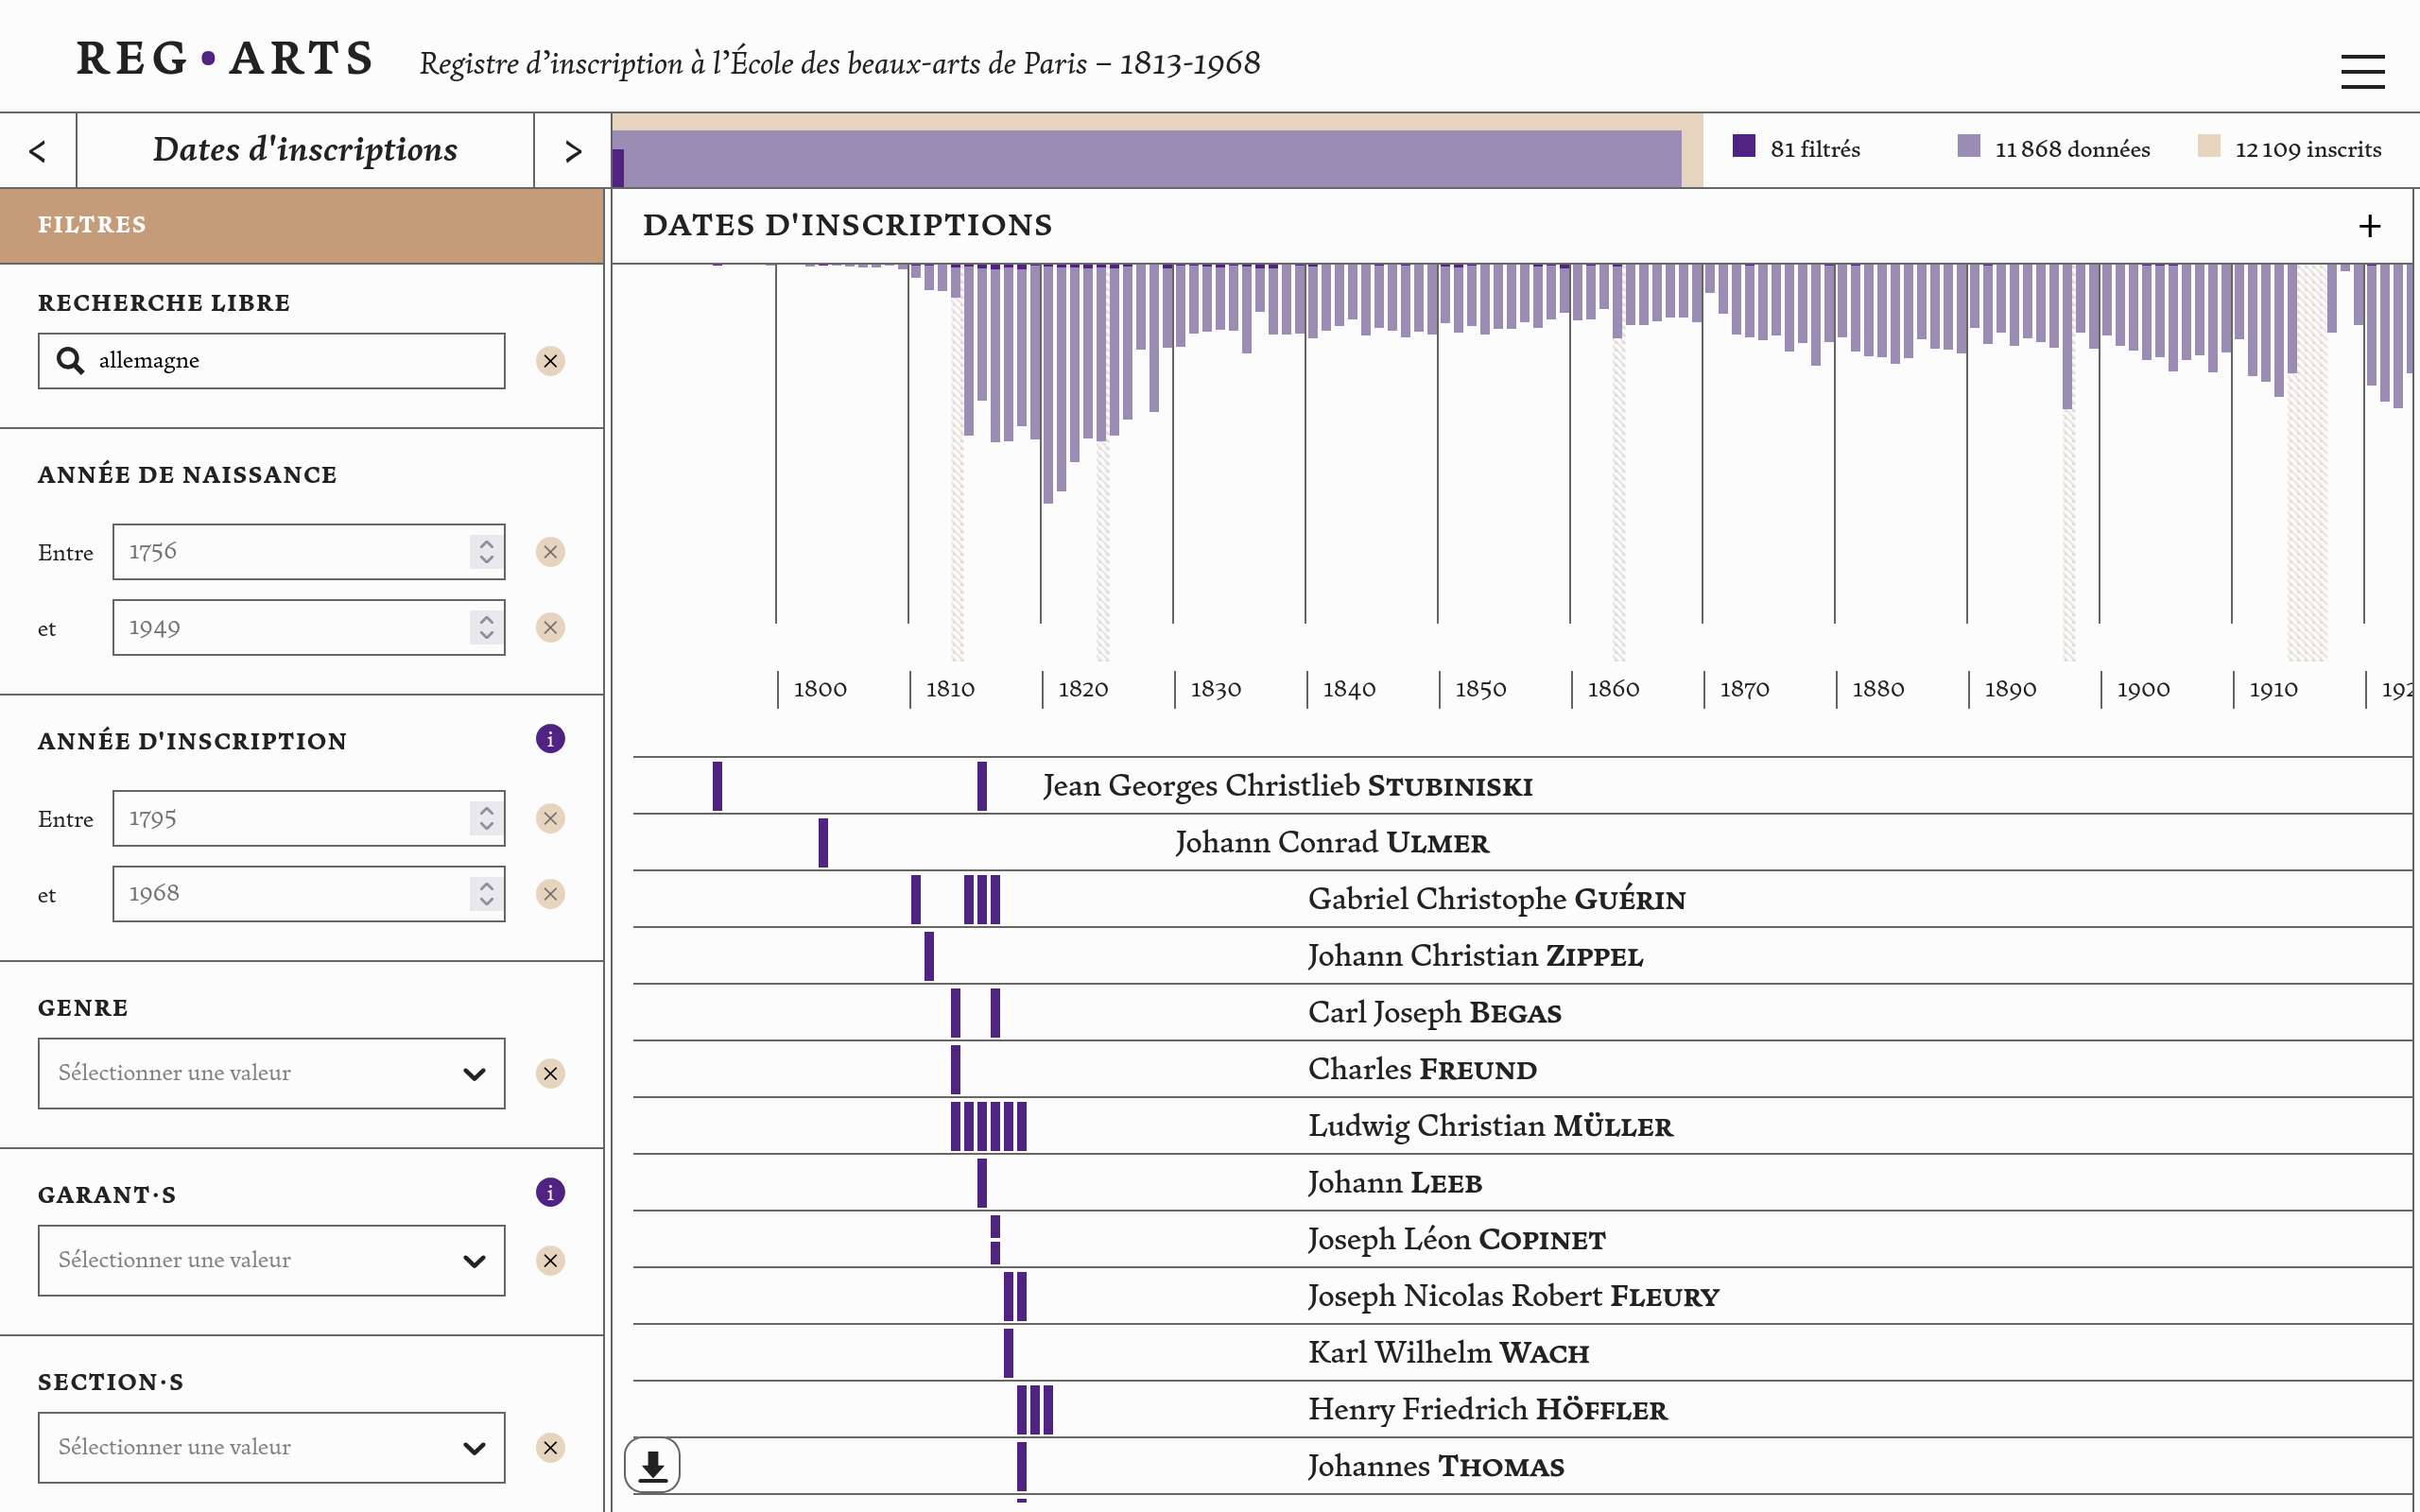
\includegraphics[width=1\linewidth]{figures/faceted_search.png}
  \caption{Students faceted search page with an active filter for “allemagne” (\href{https://regarts.huma-num.fr/v/inscriptions?fullText=allemagne}{https://regarts.huma-num.fr/v/inscriptions?fullText=allemagne}).}
  \label{fig:faceted_search}
\end{figure}

\section{Geographical Custom Static Vector Tiles}
We created two geographical maps: one displaying students’ birthplaces worldwide (1756-1949), and another showing their Parisian addresses (1813-1900). Modern JavaScript libraries such as \href{https://leafletjs.com/}{Leaflet}\footnote{https://leafletjs.com/} and \href{https://maplibre.org/}{MapLibre}\footnote{https://maplibre.org/} have greatly simplified the process of displaying data on web maps. Recently, vector tiles have emerged as an alternative to raster tiles, sending geographical data as geometries rather than images. This allows the client to customize rendering styles, whereas raster tiles require selecting a provider with a suitable basemap.

For historical maps, we needed to avoid anachronisms, such as contemporary political borders or modern infrastructure, when visualizing 19th-century data. We also wanted the basemap to integrate seamlessly with our website’s design, serving as a discreet, informative background. To satisfy these two requirements we used Vector tiles which offers the flexibility to filter geographical elements (like highways) and apply custom styles to tune colors and shapes.

However, most vector tile libraries are client-side rendering engines that depend on third-party data providers. To adhere to our no-server constraint, we used the \href{https://protomaps.com/}{Protomaps}\footnote{https://protomaps.com/} provider and the \href{https://docs.protomaps.com/pmtiles/}{\texttt{pmtiles} protocol}\footnote{https://docs.protomaps.com/pmtiles/}, which allows a client-side map renderer to query tiles using standard HTTP range requests. Serving pmtiles is as simple as hosting a single binary file on any web server.

To create our vector tiles, we first downloaded a worldwide tile-set from Protomaps, limiting the zoom level to avoid unnecessary detail:
\begin{verbatim}
pmtiles extract https://build.protomaps.com/20240912.pmtiles
                10.pmtiles --maxzoom=10
\end{verbatim}
We then filtered geographical features to remove anachronistic elements (e.g., modern borders, highways) using the \href{https://github.com/felt/tippecanoe}{tippecanoe}\footnote{We used the now deprecating version https://github.com/mapbox/tippecanoe. The active version is now the fork https://github.com/felt/tippecanoe} utility:
\begin{verbatim}
tile-join -l natural -l earth -l water -l "physical line" -l places
          -o 10_simplified.pmtiles 10.pmtiles
\end{verbatim}
The resulting \texttt{10\_simplified.pmtiles} file served as the basis for our birthplaces map.

For the Parisian addresses map, we required street-level detail and a broader context for France. We extracted and filtered tiles for France up to zoom level 10:
\begin{verbatim}
pmtiles extract https://build.protomaps.com/20240912.pmtiles France10.pmtiles
    --maxzoom=10 --bbox=-11.250000,39.334297,19.555664,55.429013
tile-join -l natural -l earth -l water -l "physical line" -l places
          -o France_10_simplified.pmtiles France_10.pmtiles
\end{verbatim}

\begin{figure}[t!]
  \centering
  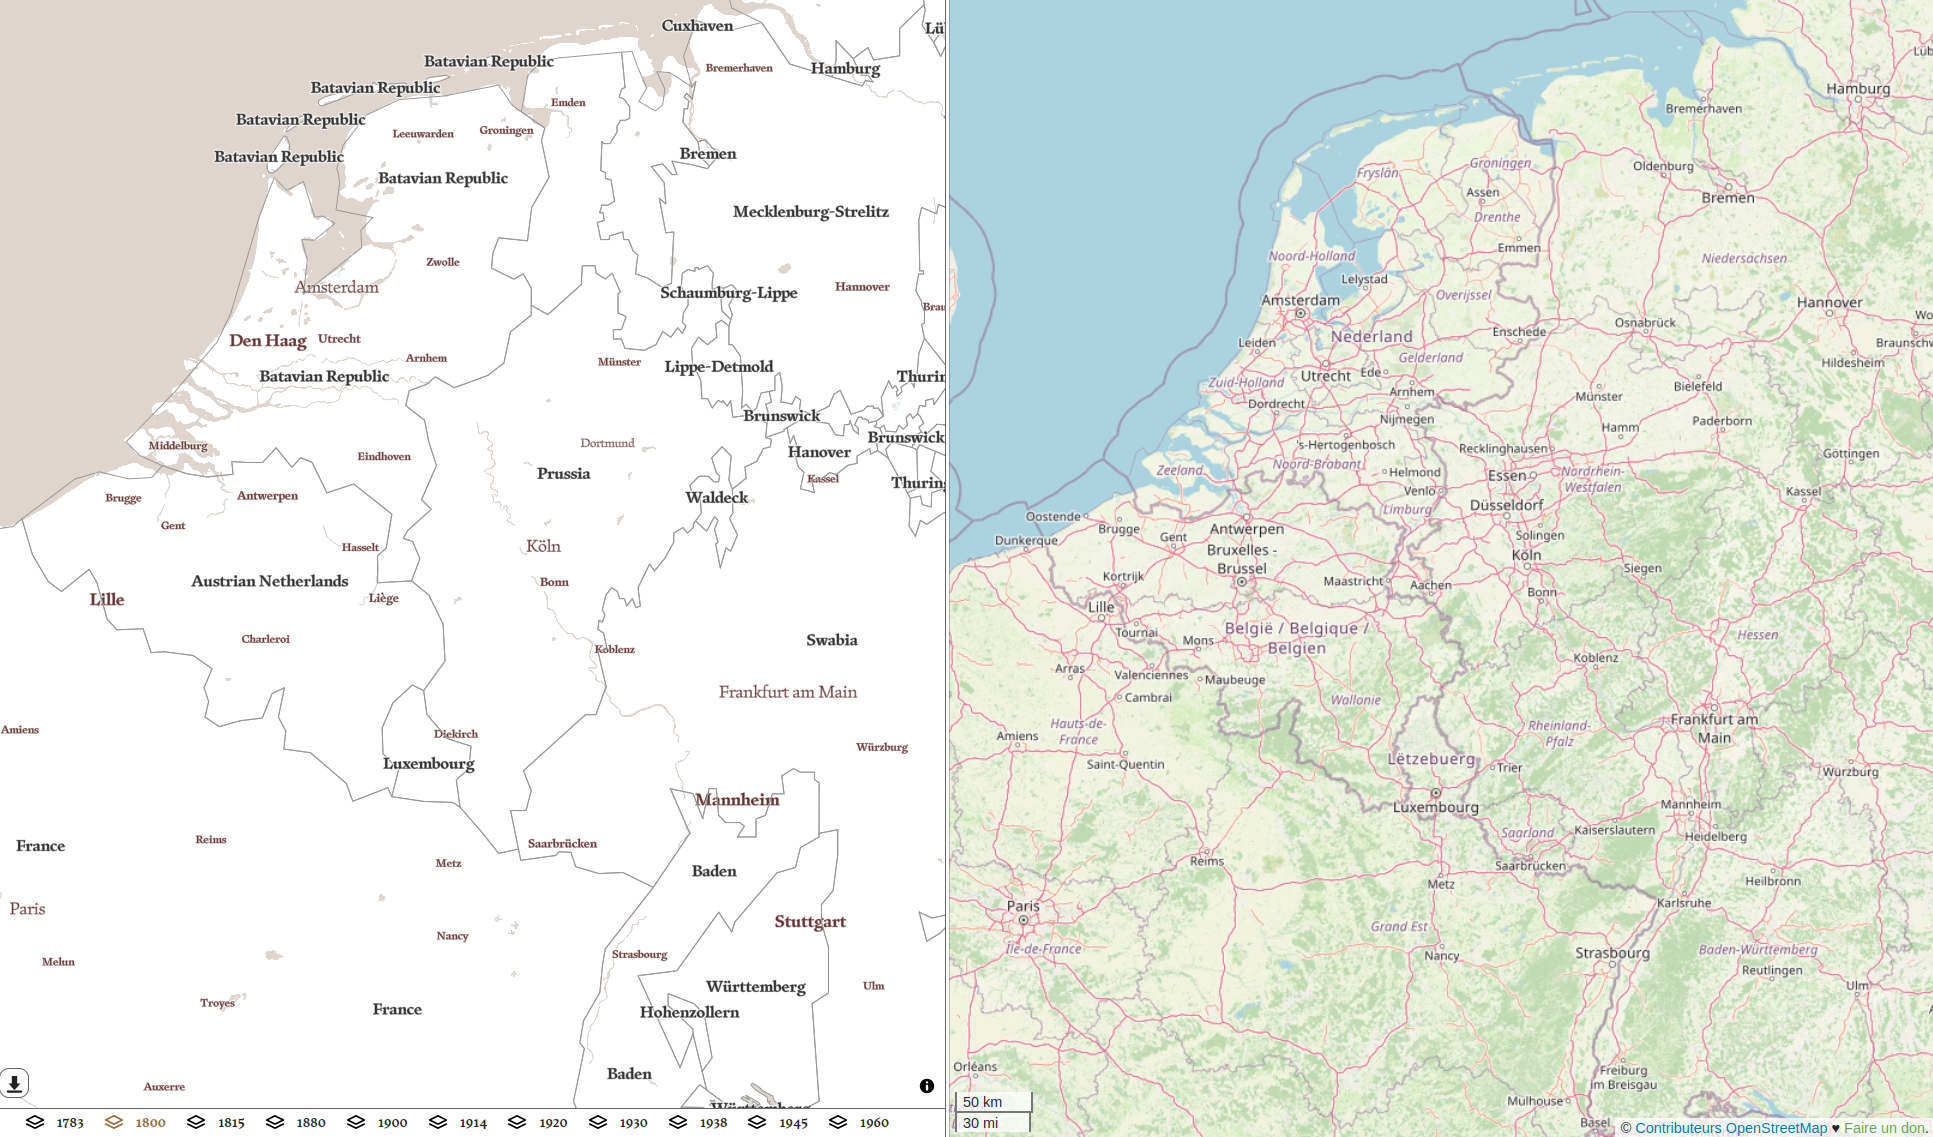
\includegraphics[width=1\linewidth]{figures/map_compared.png}
  \caption{Custom style for the birthplaces map with 1815 historical borders (left) compared to the standard OpenStreetMap style (right).}
  \label{fig:map_compared}
\end{figure}

We then created a Paris-specific tile-set, including roads, and combined it with the France tile-set:
\begin{verbatim}
pmtiles extract https://build.protomaps.com/20240912.pmtiles Paris921.pmtiles
    --maxzoom=21 --minzoom=9 --bbox=1.797638,48.622924,2.866058,49.124669
tile-join -l natural -l earth -l water -l "physical line" -l places -l roads
          -o Paris_9_21_simplified.pmtiles Paris_9_21.pmtiles
tile-join France_10_simplified.pmtiles Paris_9_21_simplified.pmtiles
          -o Paris_21_France_10.pmtiles
\end{verbatim}
By restricting areas, zoom levels, and geographical features, we minimized data size. The Paris map tile-set weighs 293 MB, while the worldwide birthplaces map is 1.9 GB—a reasonable size for global coverage. However, only the required tiles are transferred during map display.

We further enhanced the basemaps by overlaying historical borders from André Ourednik’s \href{https://github.com/aourednik/historical-basemaps}{historical-basemaps}\footnote{https://github.com/aourednik/historical-basemaps} (GeoJSON) and historical Paris street maps\footnote{Those maps are hosted by a third-party service. It's an exception from our "serverless" rule.} from Gallica BNF, processed by \href{https://ptm.huma-num.fr/}{Projets Time Machine}\footnote{https://ptm.huma-num.fr/}.



\begin{figure}[t!]
  \centering
  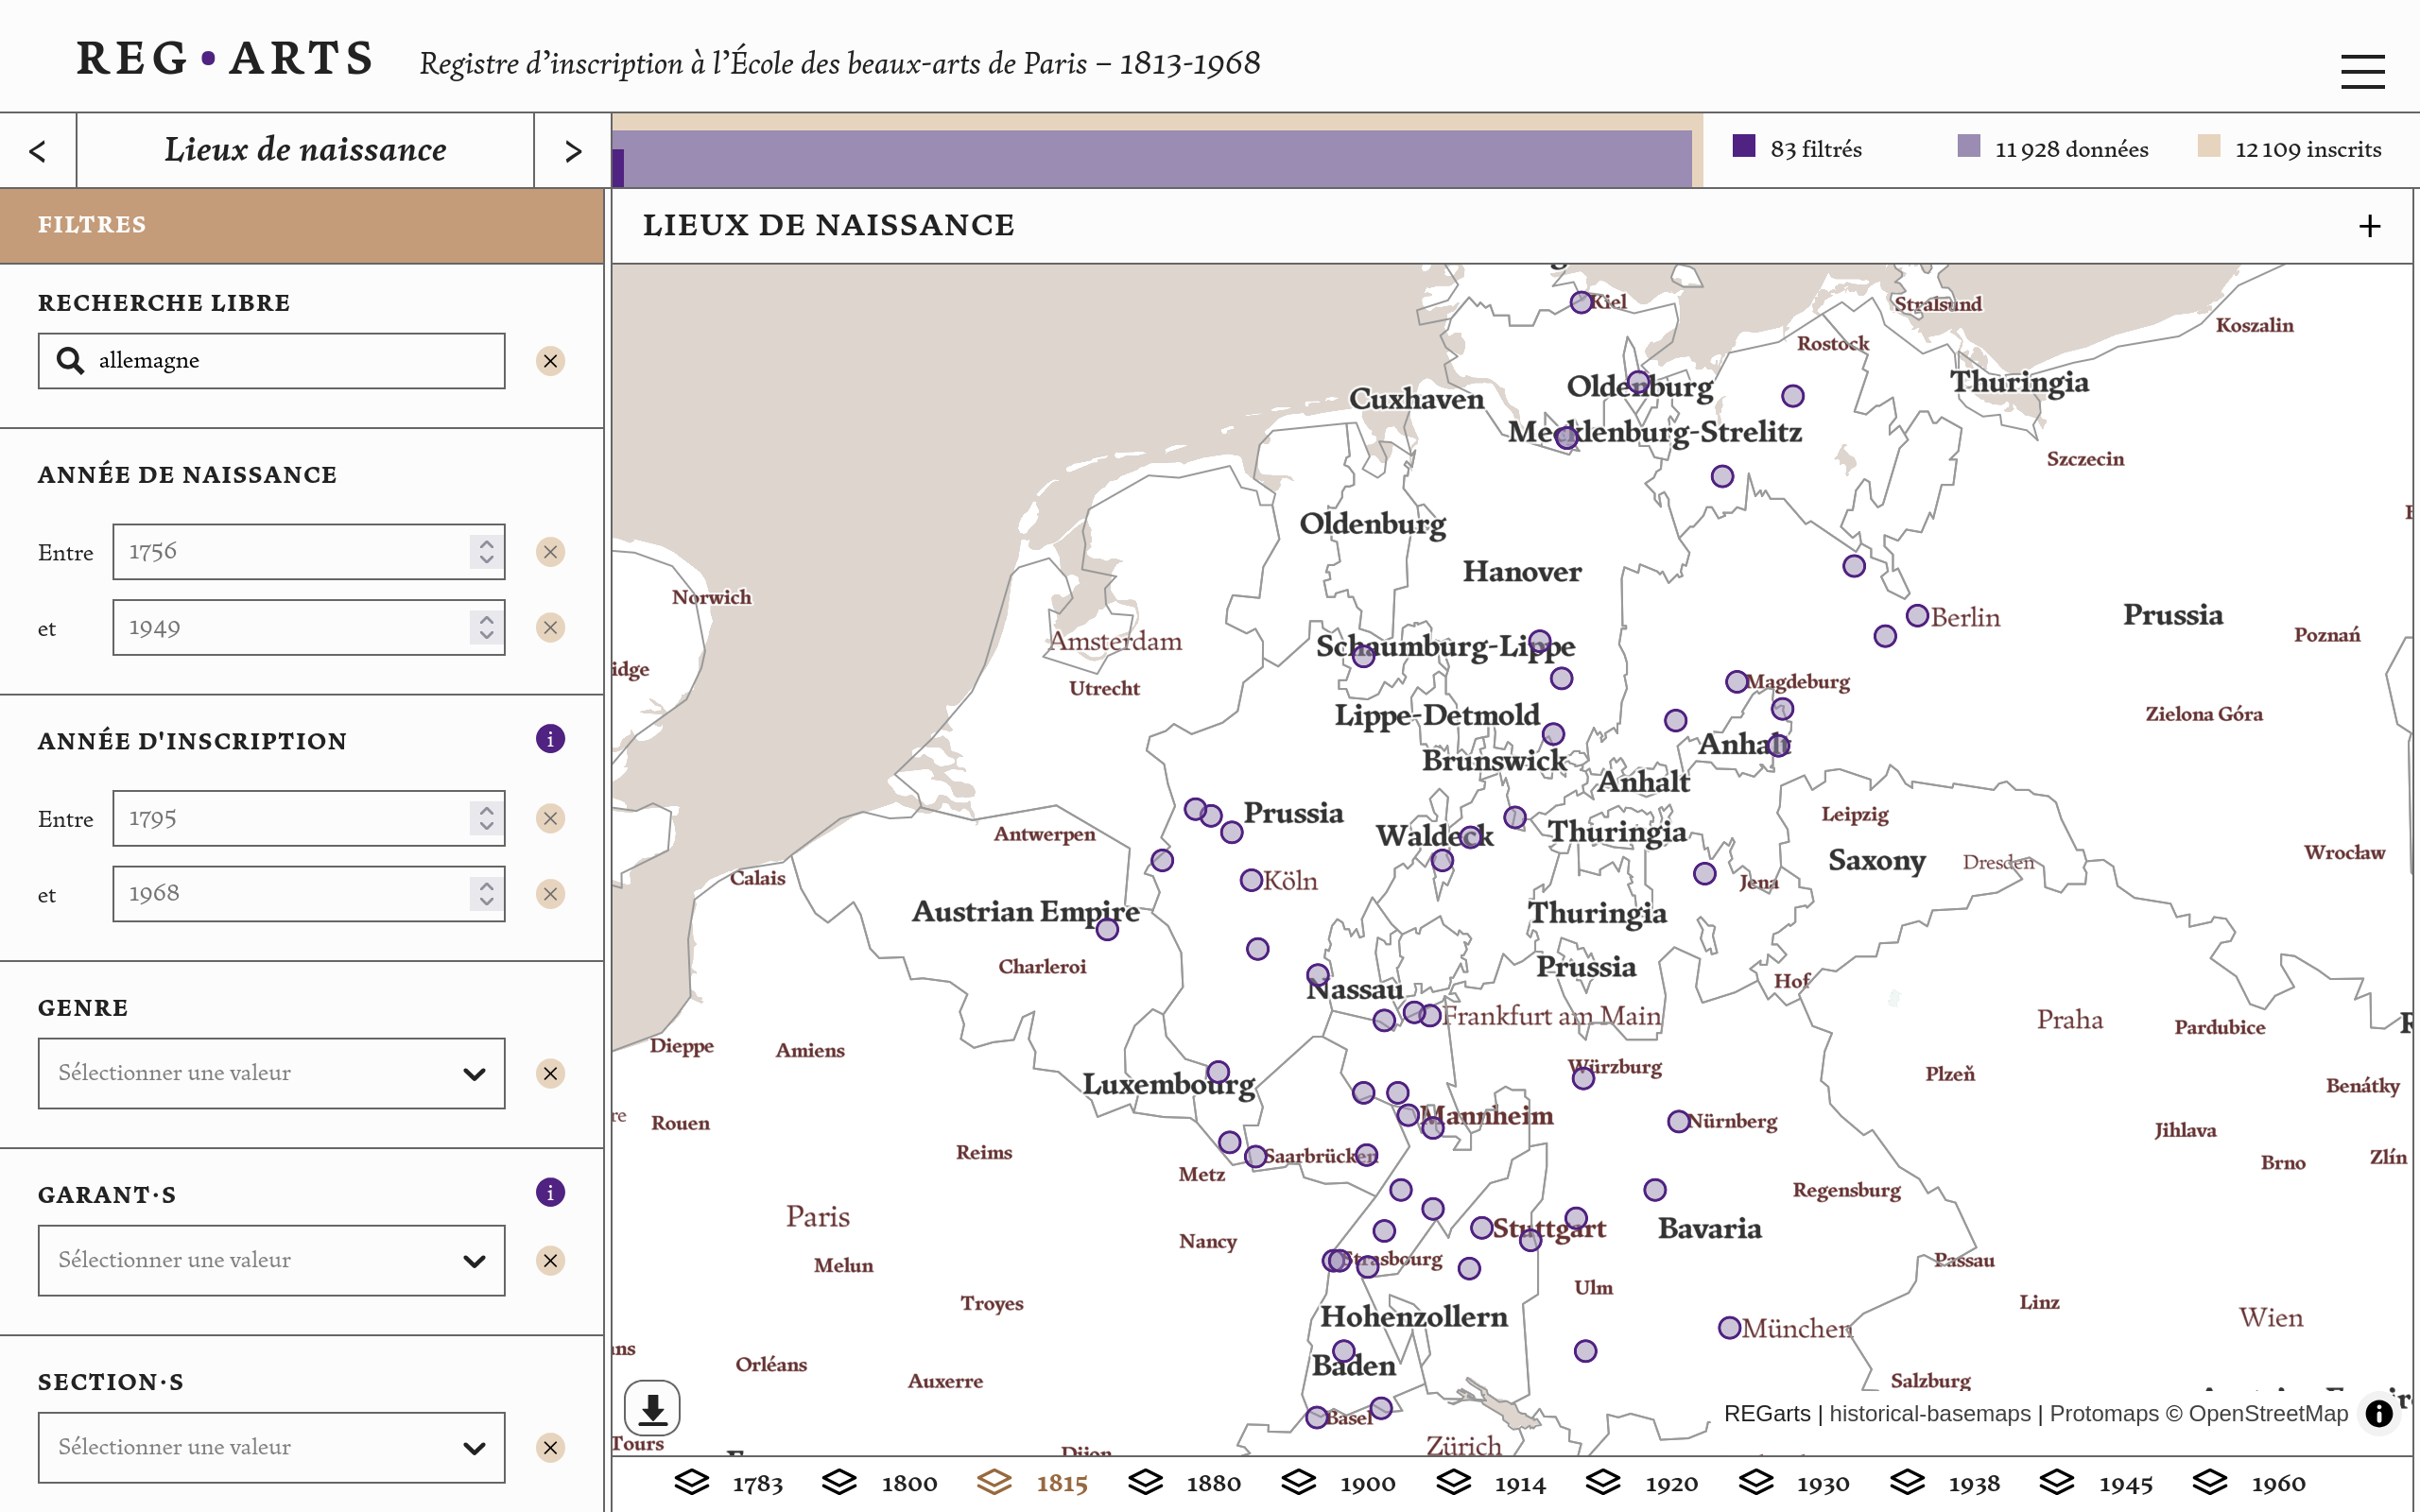
\includegraphics[width=1\linewidth]{figures/brithplaces_map.png}
  \caption{Birthplaces map with 1815 historical borders, showing students born in contemporaneous “Allemagne” (\href{https://regarts.huma-num.fr/v/naissance?fullText=allemagne}{https://regarts.huma-num.fr/v/naissance?fullText=allemagne}).}
  \label{fig:birthplaces_map}
\end{figure}

\begin{figure}[t!]
  \centering
  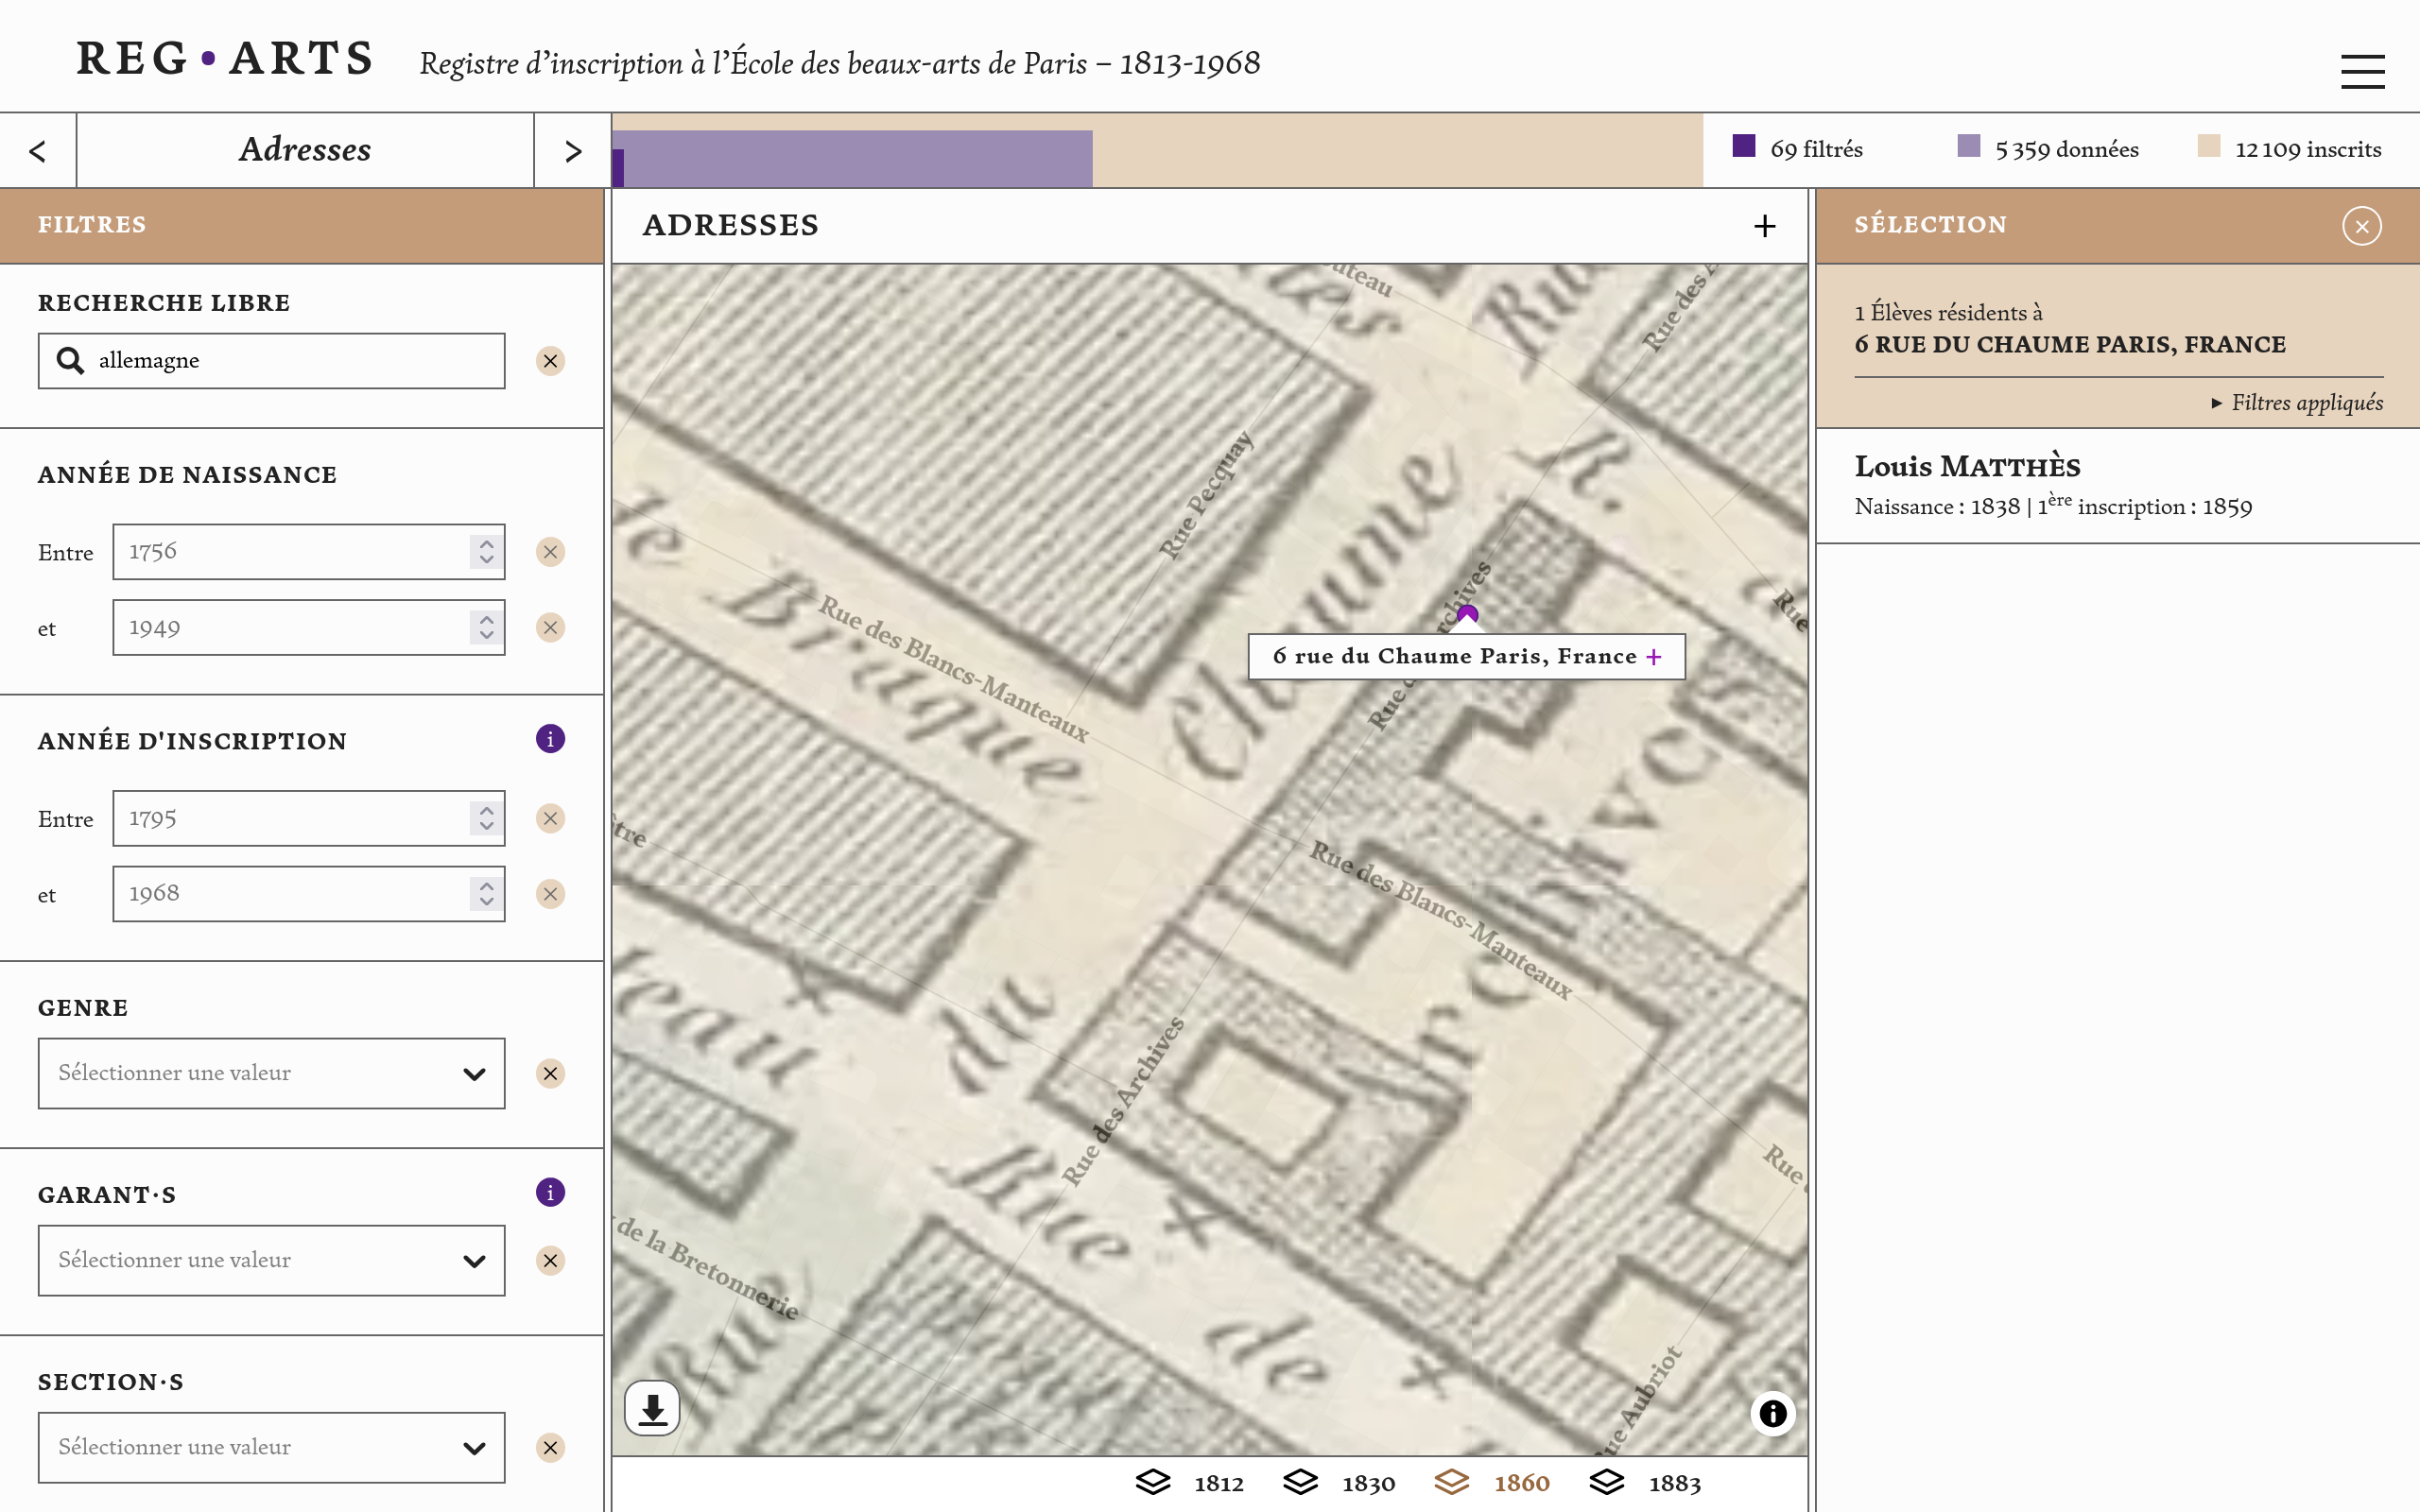
\includegraphics[width=1\linewidth]{figures/paris_map_chaume.png}
  \caption{Map of Paris showing students’ home addresses, with an overlay of an 1860 historical map indicating that “rue de Chaume” is an old name for “rue des archives” (\href{https://regarts.huma-num.fr/v/adresses?fullText=allemagne}{https://regarts.huma-num.fr/v/adresses?fullText=allemagne}).}
  \label{fig:home_map}
\end{figure}

\section{Discussion}
Our work enables exploration of the \href{https://regarts.huma-num.fr/v/naissance}{birthplaces}\footnote{https://regarts.huma-num.fr/v/naissance} and \href{https://regarts.huma-num.fr/v/adresses}{home addresses}\footnote{https://regarts.huma-num.fr/v/adresses} of students registered at the École des beaux-arts de Paris during the 19th century. A \href{https://regarts.huma-num.fr/v/reseau}{network visualization}\footnote{https://regarts.huma-num.fr/v/reseau} showing links between presenters and their recommended students, powered by the \href{https://sigmajs.org}{sigma.js library}\footnote{https://sigmajs.org}, further supports visual network analysis directly in the browser. 

Reg$\cdot$Arts web application enables users to search for individual students, whether for art historical research or related fields such as genealogy, in order to examine their trajectories at the École des Beaux-Arts. Additionally, the platform offers analytical tools and datasets for broader studies, including the demography of Parisian art students and the evolution of the school’s recruitment networks. 

While static web development may not suit all projects, it offers a compelling approach for many use cases. However, it imposes technical constraints that require adapting both usage and design. Adopting a “minimal” mindset is essential \cite{risam_introduction_2022}: it encourages data size limitations and may necessitate sacrificing advanced features. In our case fuzzy full-text search was dropped in favor of the simpler yet sufficient regex search. Developers must also ensure that scientific requirements are met; in our case, the \texttt{pmtiles} protocol allowed us to provide historically accurate basemaps while respecting our static constraints.

A major drawback of the static approach is the shift of computational and network demands to the client. Users with older hardware or high-latency connections may experience longer load times, though this is partly offset by the simplicity of the features. We hope to have demonstrated how the static approach, as a set of fruitful constraints, can lead to the design of simpler yet accurate web applications for digital humanities.

\printbibliography

\end{document}
